
%\setcounter{chapter}{4}


\begin{Large}
\noindent
{\bf Lecture 4 \newline
Linear Vector Space 3}
\end{Large}
\vspace{1 cm}

\section{Adjoint Operator}
Consider the equation
\be
|b\rangle = \hat{K} |a\rangle.
\label{eq:K}
\ee
The operator $\hat{K}$ carries the ket $|a\rangle$ to the ket $|b\rangle$. The dual of $|a\rangle$ and $|b\rangle$ are 
$\langle a|$ and $\langle b|$, respectively. The operator which carries $\langle a|$ to $\langle b|$ is called the 
adjoint of $\hat{K}$ and is denoted by $\hat{K}^{\dagger}$. Thus, in the dual space, Eq. (\ref{eq:K}) is
\be
\langle b| = \langle a |\hat{K}^{\dag}.
\label{eq:kdagger}
\ee
We summarize the situation in the figure below.
\begin{figure}[h]
\centering
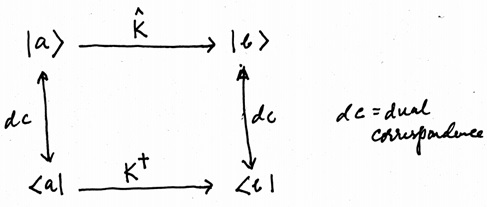
\includegraphics[width=100 mm]{adjoint.jpg}
\end{figure}

\paragraph{}
From Eqs. (\ref{eq:K}) and (\ref{eq:kdagger}) it follows that
\be
\langle c|b\rangle = \langle c|\hat{K}|a\rangle 
\ee
and
\be
\langle b|c\rangle = \langle a|\hat{K}^{\dag}|c\rangle .
\ee
Since $\langle b|c\rangle = \langle c|b\rangle^*$, we have
\be
\boxed{
\langle c|\hat{K}| a\rangle = \langle a |\hat{K}^{\dag}|c\rangle^*.
}
\label{eq:kdagger2}
\ee
Eq. (\ref{eq:kdagger2}) is the defining equation for the adjoint $\hat{K}^{\dag}$ of the operator $\hat{K}$.
In the scalar product notation (comma notation)
\[ \langle c|b\rangle \equiv (\psi_c, \psi_b) \]
Eq. (\ref{eq:kdagger2}) can be written as
\begin{eqnarray}
(\psi_c, \hat{K} \psi_a) &=& (\psi_a, \hat{K}^{\dag} \psi_c)^* \nonumber \\
&=& (\hat{K}^{\dag}\psi_c,\psi_a).
\end{eqnarray}
In particular, if we take $|c\rangle$ and $|a\rangle$ as the basis states $|i\rangle$ and $|j\rangle$, Eq. (\ref{eq:kdagger2}) 
becomes
\[ \langle i |\hat{K}|j\rangle = \langle j|\hat{K}^{\dag}|i\rangle^* \]
or,
\[ K_{ij}= \left(K^{\dag}\right)_{ji}^* \]
or,
\[ K^{\dag}_{ji}=K_{ij}^* \]
i.e.,
\[ K^{\dag}_{ij} = (K_{ji})^*.\]
In full matrix notation we can write
\be
[ \hat{K}^{\dag} ] = [ \hat{K} ]^{\dag},
\ee
where $[ \hat{K} ]$ is the matrix representation of the operator $\hat{K}$. Similarly for $\hat{K}^{\dag}$. Thus, the matrix representation
of the adjoint operator $\hat{K}^{\dagger}$ is the Hermitian conjugate of the matrix representation of $\hat{K}$.

\subsection{ Hermitian or self adjoint operator}
If $\hat{K}^{\dagger} = \hat{K}$, then $\hat{K}$ is said to be a self-adjoint or a Hermitian operator. The matrix representing
a Hermitian operaor is a Hermitian matrix i.e., 
\[ [K] =[K]^{\dag}\]
or,
\[ K_{ij}=K_{ji}^*.\]


\vspace{5 mm}
\noindent
{\bf Ex:}\newline
Show that $(\hat{A}\hat{B})^{\dag} = \hat{B}^{\dag}\hat{A}^{\dag}$.


\noindent {\bf Ans:}\newline
\be
\left(\psi_a,\hat{A}\hat{B}\psi_b\right) =\left((\hat{A}\hat{B})^{\dag}\psi_a,\psi_b\right).
\label{eq:AB1}
\ee
Also,
\be
\left(\psi_a,\hat{A}\hat{B}\psi_b\right)= \left( \hat{A}^{\dag}\psi_a,\hat{B}\psi_b\right)=
\left(\hat{B}^{\dag}\hat{A}^{\dag},\psi_b\right)
\label{eq:AB2}
\ee
Comparing Eqs. (\ref{eq:AB1}) and (\ref{eq:AB2}), we have
\be
\left( \hat{A}\hat{B}\right)^{\dag}=\hat{B}^{\dag}\hat{A}^{\dag}.
\ee


\subsection{Inverse operator}
An operator $\hat{B}$ is said to be the inverse of the operator $\hat{A}$ if
\be
\hat{A}\hat{B} = \hat{B}\hat{A}= \hat{I}.
\label{eq:inverse}
\ee
Obviously if $\hat{B}$ is the inverse of $\hat{A}$, then $\hat{A}$ is the inverse of $\hat{B}$. We write
\[ \hat{B} = \hat{A}^{-1}\]
or,
\[ \hat{A} = \hat{B}^{-1} \]
if Eq. (\ref{eq:inverse}) is satisfied.


\subsection{Unitary operator}
An operator $\hat{U}$ is said to be unitary if 
\be
\hat{U}\hat{U}^{\dag}=\hat{U}^{\dag}\hat{U} = \hat{I}
\ee
i.e., if
\be
\hat{U}^{\dag}=\hat{U}^{-1}.
\ee
Thus, for a unitary operator, its adjoint is also its inverse. 



\section{Functions of operators}
Consider a real-valued function $f(x)$ of a real variable $x$. Suppose that the function has a power series expansion 
\be
f(x) = f_0 + xf_1 + x^2 f_2 + \cdots.
\ee
If $\hat{A}$ is an operator, we can define the operator $\hat{f}(\hat{A})$ as
\be
\hat{f}(\hat{A}) = f_0 \hat{I} + \hat{A}f_1 + \hat{A}^2 f_2 + \cdots.
\ee
As an example of a function of an operator, consider the operator $e^{\lambda\hat{A}}$. This is defined as
\be
e^{\lambda\hat{A}}= \hat{I} + \lambda \hat{A} + \frac{\lambda^2}{2!} \hat{A}^2 + \frac{\lambda^3}{3!}\hat{A}^3 + \cdots.
\ee

\paragraph{}
One must be careful in manipulating functions of operators since operators do not commute with each other in general. For example,
if $\hat{A}\hat{B} \neq \hat{B}\hat{A}$, then
\be
e^{\hat{A}+\hat{B}} \neq e^{\hat{A}}e^{\hat{B}} \neq e^{\hat{B}}e^{\hat{A}}.
\ee
In the special case when $[\hat{A}, \hat{B}]$ is a number times the unit operator, i.e.,
\[ [\hat{A},\hat{B}] = c \hat{I} \]
where $c$ is a number (in general complex), then
\be
e^{\hat{A}+\hat{B}} = e^{\hat{A}}e^{\hat{B}}e^{-[\hat{A},\hat{B}]/2}.
\ee
This result is known as Weyl's identity. For example, in quantum mechanics we have
\[ [\hat{x},\hat{p}_x]=i\hbar \hat{I}. \]
So Weyl's identity would be satisfied by $\hat x$ and $\hat{p}_x$.


\vspace{5 mm}
\noindent {\bf Examples}

\noindent{\bf Ex}
Show that
\begin{equation}
e^{\lambda \hat{A}}\hat{B} e^{-\lambda \hat{A}} = \hat{B} + \lambda [\hat{A},\hat{B}] +\frac{\lambda^2}{2!}[\hat{A},[\hat{A},\hat{B}]]
+ \frac{\lambda^3}{3!}[\hat{A},[\hat{A},[\hat{A},\hat{B}]]]+ \cdots .
\end{equation}

\vspace{3 mm}
\noindent 
{\bf Ans:}\newline
Let
\[ f(\lambda)= e^{\lambda \hat{A}}\hat{B} e^{-\lambda \hat{A}}.\]
Therefore
\[
\frac{df(\lambda)}{d\lambda}= e^{\lambda \hat{A}}\hat{A}\hat{B} e^{-\lambda \hat{A}} - 
e^{\lambda \hat{A}}\hat{B}\hat{A} e^{-\lambda \hat{A}} = e^{\lambda \hat{A}}[\hat{A},\hat{B}] e^{-\lambda \hat{A}}.
\]
Differentiating one more time, we have
\[
\frac{d^2f(\lambda)}{d\lambda^2} = e^{\lambda \hat{A}}[\hat{A},[\hat{A},\hat{B}]] e^{-\lambda \hat{A}},
\]
and so on. Also
\[
f(0)=\hat{B},\;\; \left( \frac{df}{d\lambda}\right)_{\lambda = 0} =[\hat{A},\hat{B}], \;\;
\left(\frac{d^2f}{d\lambda^2}\right)_{\lambda =0} = [\hat{A},[\hat{A},\hat{B}]], \; \cdots 
\]
Expanding $f(\lambda)$ in a Taylor series:
\[
f(\lambda)=f(0) + \lambda \left( \frac{df}{d\lambda}\right)_{\lambda = 0} + 
\frac{\lambda^2}{2!} \left(\frac{d^2f}{d\lambda^2}\right)_{\lambda =0}+ \cdots
\]
we have
\[
e^{\lambda \hat{A}}\hat{B} e^{-\lambda \hat{A}} = \hat{B} + \lambda [\hat{A},\hat{B}] +\frac{\lambda^2}{2!}[\hat{A},[\hat{A},\hat{B}]]
+  \cdots .
\]


\section{Change of basis}
Supose we have a set of complete orthonormal basis set $\{|u_i\rangle\}$ in a Hilbert space. The orthonormality and completeness of the 
vasis set can be expressed as
\be
\langle u_i|u_j\rangle = \delta_{ij} \;\; {\text{orthonormality}}
\ee
and
\be 
\sum_i |u_i\rangle \langle u_i| = \hat{I}\;\; {\text{completeness}}.
\ee
In terms of the basis set $\{ |u_i\rangle \}$, an arbitrary ket $|\psi\rangle$ of the Hilbert space can be expanded as
\be
|\psi\rangle = \sum_i |u_i\rangle \langle u_i|\psi\rangle = \sum_i a_i |u_i\rangle,
\ee
where
\be
a_i= \langle u_1|\psi\rangle
\ee
is the component of $|\psi\rangle$ along $|u_i\rangle$. The numbers $a_i$ arranged as a column matrix is called the representation
of the ket $|\psi\rangle$ in the basis $\{ |u_i\rangle\}$.
Thus,
\be
|\psi\rangle \longrightarrow \begin{bmatrix} a_1\\a_2\\\vdots \end{bmatrix}
= \begin{bmatrix} \langle u_1|\psi\rangle \\\langle u_2|\psi\\\vdots \end{bmatrix}.
\ee
The conjugate of $|\psi\rangle$ in the dual space is written as the bra $\langle \psi|$. The matrix representation of 
$\langle \psi|$ is the row vector with components $\langle \psi|u_i\rangle$, i.e. $\langle u_i|\psi \rangle ^*$. Thus,
\be
\langle \psi| \longrightarrow \begin{bmatrix} \langle \psi|u_1\rangle & \langle \psi|u_2\rangle & \cdots \end{bmatrix}
= \begin{bmatrix} a_1^* & a_2^* & \cdots \end{bmatrix}.
\ee

\paragraph{}
Using the basis $\{ |u_i\rangle\}$, we can also write down the representation of an operator $\hat{A}$ as a square
matrix with elements $A_{ij}$ given by
\be
A_{ij}=\langle u_i|\hat{A}|u_j\rangle.
\ee
Writing in full 
\be
\hat{A} \rightarrow [A] = \begin{bmatrix}
A_{11} & A_{12} & A_{13} & \cdots \\
A_{21} & A_{22} & A_{23} & \cdots \\
A_{31} & A_{32} & A_{33} & \cdots \\
\vdots & \vdots & \vdots & \vdots
\end{bmatrix} 
\ee

\paragraph{}
Now, we make a change from the basis vectors $\{ |u_i\rangle, i=1,2,3, \cdots \}$ to a new set of orthonormal basis vectors
$\{ |u_i^{\prime}\rangle, i=1,2,3, \cdots \}$. The orthonormality and completeness of the new basis states can be expressed as
\be
 \langle u_i^{\prime}|u_i^{\prime}\rangle = \delta_{ij}
\ee
and
\be
\sum_i |u_i^{\prime}\rangle \langle u_i^{\prime}| = \hat{I}.
\ee
We can also write down the matrix representations of kets and operators in the new basis. We want to find how the components of the
ket $|\psi\rangle$ in the new basis relates to the components in the old basis. Similarly, we also want to know how the matrix
elements of an operator transform as we make the change of basis.


\subsection{Change of representation for kets}
Let $|\psi\rangle$ be an arbitrary ket in the vector space $V$. In the new basis $\{ |u_i^{\prime}\rangle \}$, the components
$a_i^{\prime}$ of the ket $|\psi\rangle$ are
\begin{eqnarray}
a_i^{\prime} &=& \langle u_i^{\prime}|\psi \rangle \nonumber \\
&=& \sum_j \langle u_i^{\prime}|u_j\rangle \langle u_j|\psi\rangle, 
\end{eqnarray}
or,
\be
a_i^{\prime} = \sum_j S_{ij}a_j
\label{eq:ket}
\ee
where we have defined
\be
S_{ij}= \langle u_i^{\prime}|u_j\rangle.
\ee
In matrix form Eq. (\ref{eq:ket}) is
\be
\begin{bmatrix} a_1^{\prime} \\ a_2^{\prime}\\ \vdots \end{bmatrix} =
\begin{bmatrix}
\langle u_1^{\prime}|u_1\rangle & \langle u_1^{\prime}|u_2\rangle & \hdots \\
\langle u_2^{\prime}|u_1\rangle & \langle u_2^{\prime}|u_2\rangle & \hdots \\
\vdots                          & \vdots                          & \vdots
\end{bmatrix}
\begin{bmatrix} a_1 \\ a_2 \\ \vdots \end{bmatrix}.
\ee
Before proceeding, we shall show that the matrix $[S] =(S_{ij})$ is unitary.

\subsubsection{To show that $[S]$ is unitary}

We start with the orthonormality of the new basis set, i.e., 
\[ \langle u_i^{\prime}|u_j^{\prime}\rangle = \delta_{ij} \]
or,
\[ \sum_k \langle u_i^{\prime}|u_k\rangle \langle u_k|u_j^{\prime}\rangle =\delta_{ij}, \]
or,
\[ \sum_k S_{ik}S_{jk}^* = \delta_{ij}, \]
or,
\[ \sum_{k} S_{ik}S^{\dag}_{kj} =\delta_{ij} \]
i.e.,
\[ [S][S]^{\dag} = [I].\]
Next, we use the orthonormality of the old basis set.
\[ \langle u_i|u_j\rangle = \delta_{ij} \]
or,
\[ \sum_k \langle u_i|u_k^{\prime}\rangle \langle u_k^{\prime}|u_j\rangle =\delta_{ij}, \]
or,
\[ \sum_k S^*_{ki}S_{kj} = \delta_{ij}, \]
or,
\[ \sum_{k} S^{\dag}_{ik}S_{kj} =\delta_{ij} \]
i.e.,
\[ [S]^{\dag}[S] = [I].\]
Thus, we have proved
\be
[S][S]^{\dag}= [S]^{\dag}[S] = [I],
\ee
i.e.,
$[S]$ is a unitary matrix.



\section{Transformation of the matrix elements of an operator due to a change of basis}
Next, we will discuss how the matrix elements of an operator transform if we make a change of basis. To do so, we proceed as follows.
\begin{eqnarray}
A^{\prime}_{ij} &=& \langle u_i^{\prime}|\hat{A}|u_j^{\prime}\rangle \nonumber \\
&=& \sum_{k,l} \langle u_i^{\prime}|u_k\rangle \langle u_k|\hat{A}|u_l\rangle \langle u_l|u_j^{\prime}\rangle \nonumber \\
&=& \sum_{k,l} \langle u_i^{\prime}|u_k\rangle A_{kl} \langle u_j^{\prime}|u_l\rangle^* \nonumber \\
&=& \sum_{k,l} S_{ik}A_{kl}S_{jl}^* .
\end{eqnarray} 
In the full matrix notation we can write
\be
[A]^{\prime} = [S][A][S]^{\dag} , 
\ee
or, since $[S]$ is unitary,
\be
[A]^{\prime} = [S][A][S]^{-1}.
\ee
Such a transformation of a square matrix is called a similarity transformation.



